\subsection{Experiment 1}
\label{ssec:exp1}
\addcontentsline{toc}{section}{Experiment 1}

In this experiment we determine how the size of thethe gap determines the minimum number of
bots needed to cross over the gap. The minimum number of bots needed to perform
a task with certain paramters can be determined from the ratio of succesfull to
unsuccesfull runs with these runs with these run. In this experiment there is
one box with a weight of one. The number of bots varies from 1 to 20.

The graph of runs with a gap size of 0, 3, 4 and 10 can be seen in
figure~\ref{fig:exp1-graphs}, the graphs the other size look similar. We see
that the number of bots needed increases with the gap size up to a gap size of
4. From a gap size of 4 onwards the number of bots needed remains 6. In the
simulation we see the group of bots moving over the floor of the gap, without
trying to fill the whole gap.

\begin{figure}
\subfloat[Gap size 0]{
    \label{fig:exp1-graphs:0}
    \begin{minipage}[b]{0.5\linewidth}
    \centering
    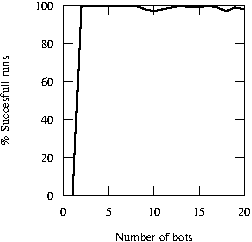
\includegraphics[width=\linewidth]{results/experiment1/plot0}
    \end{minipage}
}%
\hfill
\subfloat[Gap size 3]{
    \label{fig:exp1-graphs:3}
    \begin{minipage}[b]{0.5\linewidth}
    \centering
    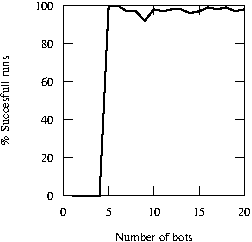
\includegraphics[width=\linewidth]{results/experiment1/plot3}
    \end{minipage}
}

\subfloat[Gap size 4]{
    \label{fig:exp1-graphs:4}
    \begin{minipage}[b]{0.5\linewidth}
    \centering
    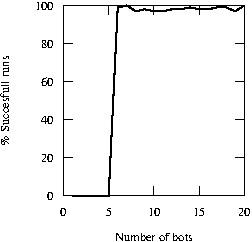
\includegraphics[width=\linewidth]{results/experiment1/plot4}
    \end{minipage}
}%
\hfill
\subfloat[Gap size 10]{
    \label{fig:exp1-graphs:10}
    \begin{minipage}[b]{0.5\linewidth}
    \centering
    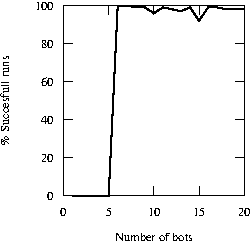
\includegraphics[width=\linewidth]{results/experiment1/plot10}
    \end{minipage}
}

\caption{Succesrate and number of bots for different gap sizes}
\label{fig:exp1-graphs}

\end{figure}

\begin{table}
 \caption{The variables involved in experiment 1.}
 \begin{center}
  \begin{tabular}{| p{5cm} | c | c |}
   \hline
   \centering \textbf{Variable} & \textbf{Type} & \textbf{Interval} \\ \hline
   gap size & independent & $[0, 10]$ \\ \hline
   box weight & independent & $1$ \\ \hline
   number of bots & independent & $[1, 20]$ \\ \hline
   ratio of succesfull runs & dependent &  \\ \hline
   runs per parameter set & other & $100$ \\ \hline
  \end{tabular}
 \end{center}
 \label{tbl:exp1}
\end{table}
